% Created by tikzDevice version 0.12.6 on 2024-11-13 12:24:11
% !TEX encoding = UTF-8 Unicode
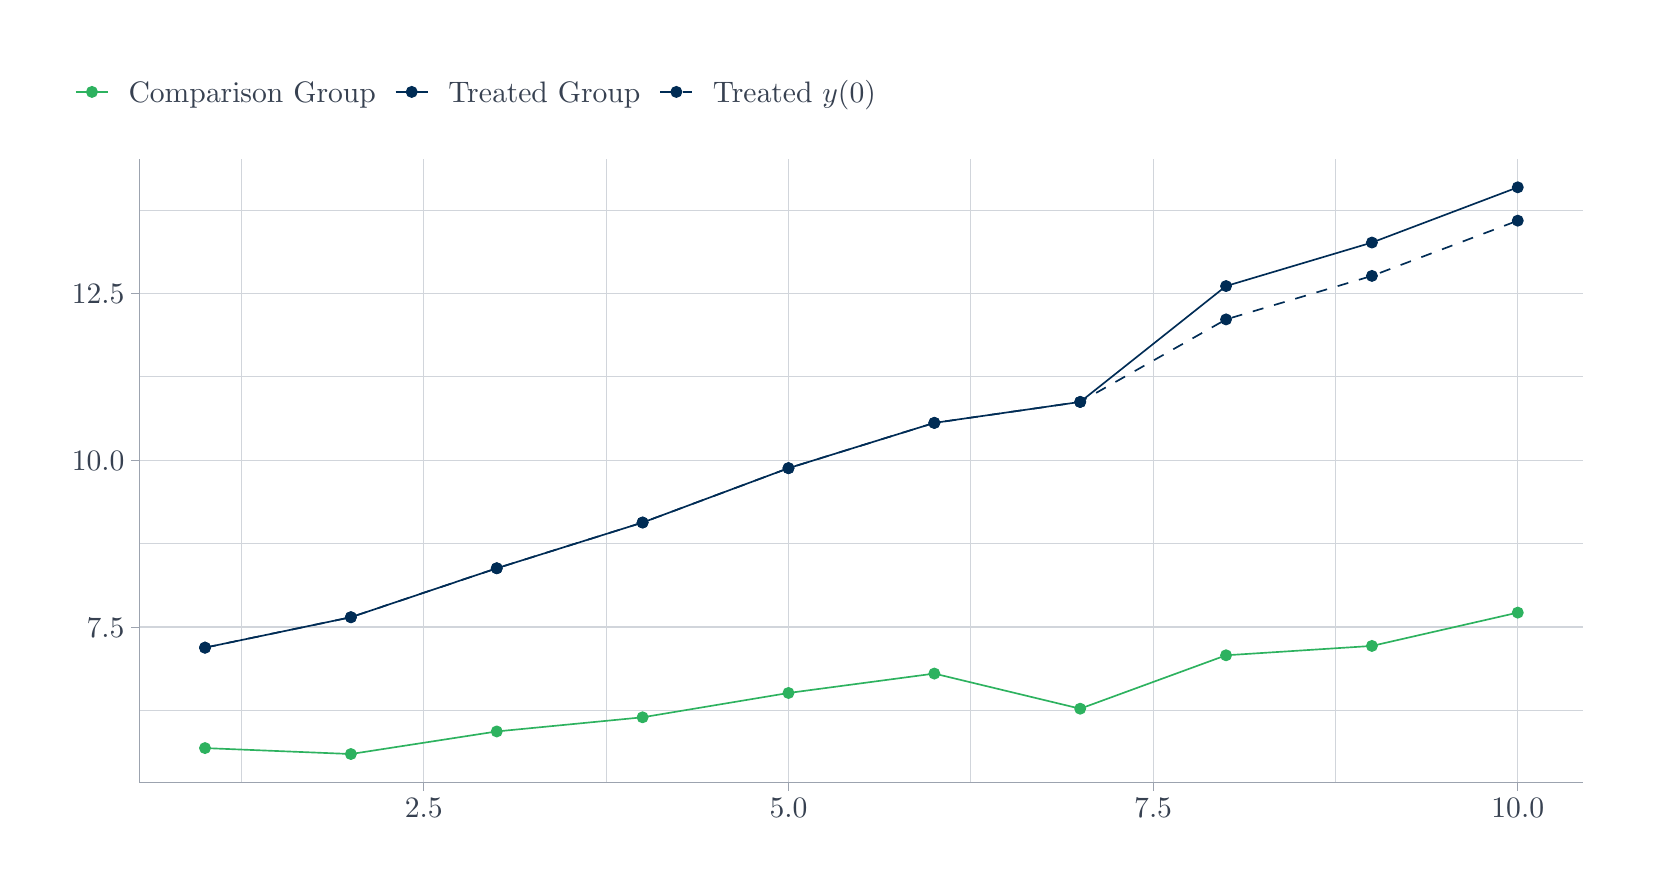
\begin{tikzpicture}[x=1pt,y=1pt]
\definecolor{fillColor}{RGB}{255,255,255}
\path[use as bounding box,fill=fillColor] (0,0) rectangle (578.16,303.53);
\begin{scope}
\path[clip] (  0.00,  0.00) rectangle (578.16,303.53);
\definecolor{drawColor}{RGB}{255,255,255}

\path[draw=drawColor,line width= 0.6pt,line join=round,line cap=round,fill=fillColor] (  0.00,  0.00) rectangle (578.16,303.53);
\end{scope}
\begin{scope}
\path[clip] ( 40.36, 30.82) rectangle (562.16,256.08);
\definecolor{drawColor}{RGB}{255,255,255}
\definecolor{fillColor}{RGB}{255,255,255}

\path[draw=drawColor,line width= 0.6pt,line join=round,line cap=round,fill=fillColor] ( 40.36, 30.82) rectangle (562.16,256.08);
\definecolor{drawColor}{RGB}{209,213,219}

\path[draw=drawColor,line width= 0.4pt,line join=round] ( 40.36, 56.85) --
	(562.16, 56.85);

\path[draw=drawColor,line width= 0.4pt,line join=round] ( 40.36,117.10) --
	(562.16,117.10);

\path[draw=drawColor,line width= 0.4pt,line join=round] ( 40.36,177.36) --
	(562.16,177.36);

\path[draw=drawColor,line width= 0.4pt,line join=round] ( 40.36,237.62) --
	(562.16,237.62);

\path[draw=drawColor,line width= 0.4pt,line join=round] ( 77.26, 30.82) --
	( 77.26,256.08);

\path[draw=drawColor,line width= 0.4pt,line join=round] (209.03, 30.82) --
	(209.03,256.08);

\path[draw=drawColor,line width= 0.4pt,line join=round] (340.79, 30.82) --
	(340.79,256.08);

\path[draw=drawColor,line width= 0.4pt,line join=round] (472.56, 30.82) --
	(472.56,256.08);

\path[draw=drawColor,line width= 0.4pt,line join=round] ( 40.36, 86.98) --
	(562.16, 86.98);

\path[draw=drawColor,line width= 0.4pt,line join=round] ( 40.36,147.23) --
	(562.16,147.23);

\path[draw=drawColor,line width= 0.4pt,line join=round] ( 40.36,207.49) --
	(562.16,207.49);

\path[draw=drawColor,line width= 0.4pt,line join=round] (143.14, 30.82) --
	(143.14,256.08);

\path[draw=drawColor,line width= 0.4pt,line join=round] (274.91, 30.82) --
	(274.91,256.08);

\path[draw=drawColor,line width= 0.4pt,line join=round] (406.68, 30.82) --
	(406.68,256.08);

\path[draw=drawColor,line width= 0.4pt,line join=round] (538.44, 30.82) --
	(538.44,256.08);
\definecolor{drawColor}{RGB}{45,178,95}

\path[draw=drawColor,line width= 0.6pt,line join=round] ( 64.08, 43.21) --
	(116.79, 41.06) --
	(169.50, 49.22) --
	(222.20, 54.33) --
	(274.91, 63.12) --
	(327.62, 70.13) --
	(380.32, 57.44) --
	(433.03, 76.74) --
	(485.74, 80.12) --
	(538.44, 92.16);
\definecolor{fillColor}{RGB}{45,178,95}

\path[draw=drawColor,line width= 0.4pt,line join=round,line cap=round,fill=fillColor] ( 64.08, 43.21) circle (  1.96);

\path[draw=drawColor,line width= 0.4pt,line join=round,line cap=round,fill=fillColor] (116.79, 41.06) circle (  1.96);

\path[draw=drawColor,line width= 0.4pt,line join=round,line cap=round,fill=fillColor] (169.50, 49.22) circle (  1.96);

\path[draw=drawColor,line width= 0.4pt,line join=round,line cap=round,fill=fillColor] (222.20, 54.33) circle (  1.96);

\path[draw=drawColor,line width= 0.4pt,line join=round,line cap=round,fill=fillColor] (274.91, 63.12) circle (  1.96);

\path[draw=drawColor,line width= 0.4pt,line join=round,line cap=round,fill=fillColor] (327.62, 70.13) circle (  1.96);

\path[draw=drawColor,line width= 0.4pt,line join=round,line cap=round,fill=fillColor] (380.32, 57.44) circle (  1.96);

\path[draw=drawColor,line width= 0.4pt,line join=round,line cap=round,fill=fillColor] (433.03, 76.74) circle (  1.96);

\path[draw=drawColor,line width= 0.4pt,line join=round,line cap=round,fill=fillColor] (485.74, 80.12) circle (  1.96);

\path[draw=drawColor,line width= 0.4pt,line join=round,line cap=round,fill=fillColor] (538.44, 92.16) circle (  1.96);
\definecolor{drawColor}{RGB}{0,44,85}

\path[draw=drawColor,line width= 0.6pt,line join=round] ( 64.08, 79.50) --
	(116.79, 90.49) --
	(169.50,108.18) --
	(222.20,124.71) --
	(274.91,144.35) --
	(327.62,160.72) --
	(380.32,168.29) --
	(433.03,210.16) --
	(485.74,225.88) --
	(538.44,245.84);
\definecolor{fillColor}{RGB}{0,44,85}

\path[draw=drawColor,line width= 0.4pt,line join=round,line cap=round,fill=fillColor] ( 64.08, 79.50) circle (  1.96);

\path[draw=drawColor,line width= 0.4pt,line join=round,line cap=round,fill=fillColor] (116.79, 90.49) circle (  1.96);

\path[draw=drawColor,line width= 0.4pt,line join=round,line cap=round,fill=fillColor] (169.50,108.18) circle (  1.96);

\path[draw=drawColor,line width= 0.4pt,line join=round,line cap=round,fill=fillColor] (222.20,124.71) circle (  1.96);

\path[draw=drawColor,line width= 0.4pt,line join=round,line cap=round,fill=fillColor] (274.91,144.35) circle (  1.96);

\path[draw=drawColor,line width= 0.4pt,line join=round,line cap=round,fill=fillColor] (327.62,160.72) circle (  1.96);

\path[draw=drawColor,line width= 0.4pt,line join=round,line cap=round,fill=fillColor] (380.32,168.29) circle (  1.96);

\path[draw=drawColor,line width= 0.4pt,line join=round,line cap=round,fill=fillColor] (433.03,210.16) circle (  1.96);

\path[draw=drawColor,line width= 0.4pt,line join=round,line cap=round,fill=fillColor] (485.74,225.88) circle (  1.96);

\path[draw=drawColor,line width= 0.4pt,line join=round,line cap=round,fill=fillColor] (538.44,245.84) circle (  1.96);

\path[draw=drawColor,line width= 0.6pt,dash pattern=on 4pt off 4pt ,line join=round] ( 64.08, 79.50) --
	(116.79, 90.49) --
	(169.50,108.18) --
	(222.20,124.71) --
	(274.91,144.35) --
	(327.62,160.72) --
	(380.32,168.29) --
	(433.03,198.11) --
	(485.74,213.83) --
	(538.44,233.79);

\path[draw=drawColor,line width= 0.4pt,line join=round,line cap=round,fill=fillColor] ( 64.08, 79.50) circle (  1.96);

\path[draw=drawColor,line width= 0.4pt,line join=round,line cap=round,fill=fillColor] (116.79, 90.49) circle (  1.96);

\path[draw=drawColor,line width= 0.4pt,line join=round,line cap=round,fill=fillColor] (169.50,108.18) circle (  1.96);

\path[draw=drawColor,line width= 0.4pt,line join=round,line cap=round,fill=fillColor] (222.20,124.71) circle (  1.96);

\path[draw=drawColor,line width= 0.4pt,line join=round,line cap=round,fill=fillColor] (274.91,144.35) circle (  1.96);

\path[draw=drawColor,line width= 0.4pt,line join=round,line cap=round,fill=fillColor] (327.62,160.72) circle (  1.96);

\path[draw=drawColor,line width= 0.4pt,line join=round,line cap=round,fill=fillColor] (380.32,168.29) circle (  1.96);

\path[draw=drawColor,line width= 0.4pt,line join=round,line cap=round,fill=fillColor] (433.03,198.11) circle (  1.96);

\path[draw=drawColor,line width= 0.4pt,line join=round,line cap=round,fill=fillColor] (485.74,213.83) circle (  1.96);

\path[draw=drawColor,line width= 0.4pt,line join=round,line cap=round,fill=fillColor] (538.44,233.79) circle (  1.96);
\end{scope}
\begin{scope}
\path[clip] (  0.00,  0.00) rectangle (578.16,303.53);
\definecolor{drawColor}{RGB}{156,163,175}

\path[draw=drawColor,line width= 0.3pt,line join=round] ( 40.36, 30.82) --
	( 40.36,256.08);
\end{scope}
\begin{scope}
\path[clip] (  0.00,  0.00) rectangle (578.16,303.53);
\definecolor{drawColor}{RGB}{55,65,81}

\node[text=drawColor,anchor=base east,inner sep=0pt, outer sep=0pt, scale=  1.07] at ( 34.96, 83.30) {7.5};

\node[text=drawColor,anchor=base east,inner sep=0pt, outer sep=0pt, scale=  1.07] at ( 34.96,143.56) {10.0};

\node[text=drawColor,anchor=base east,inner sep=0pt, outer sep=0pt, scale=  1.07] at ( 34.96,203.81) {12.5};
\end{scope}
\begin{scope}
\path[clip] (  0.00,  0.00) rectangle (578.16,303.53);
\definecolor{drawColor}{RGB}{156,163,175}

\path[draw=drawColor,line width= 0.3pt,line join=round] ( 37.36, 86.98) --
	( 40.36, 86.98);

\path[draw=drawColor,line width= 0.3pt,line join=round] ( 37.36,147.23) --
	( 40.36,147.23);

\path[draw=drawColor,line width= 0.3pt,line join=round] ( 37.36,207.49) --
	( 40.36,207.49);
\end{scope}
\begin{scope}
\path[clip] (  0.00,  0.00) rectangle (578.16,303.53);
\definecolor{drawColor}{RGB}{156,163,175}

\path[draw=drawColor,line width= 0.3pt,line join=round] ( 40.36, 30.82) --
	(562.16, 30.82);
\end{scope}
\begin{scope}
\path[clip] (  0.00,  0.00) rectangle (578.16,303.53);
\definecolor{drawColor}{RGB}{156,163,175}

\path[draw=drawColor,line width= 0.3pt,line join=round] (143.14, 27.82) --
	(143.14, 30.82);

\path[draw=drawColor,line width= 0.3pt,line join=round] (274.91, 27.82) --
	(274.91, 30.82);

\path[draw=drawColor,line width= 0.3pt,line join=round] (406.68, 27.82) --
	(406.68, 30.82);

\path[draw=drawColor,line width= 0.3pt,line join=round] (538.44, 27.82) --
	(538.44, 30.82);
\end{scope}
\begin{scope}
\path[clip] (  0.00,  0.00) rectangle (578.16,303.53);
\definecolor{drawColor}{RGB}{55,65,81}

\node[text=drawColor,anchor=base,inner sep=0pt, outer sep=0pt, scale=  1.07] at (143.14, 18.07) {2.5};

\node[text=drawColor,anchor=base,inner sep=0pt, outer sep=0pt, scale=  1.07] at (274.91, 18.07) {5.0};

\node[text=drawColor,anchor=base,inner sep=0pt, outer sep=0pt, scale=  1.07] at (406.68, 18.07) {7.5};

\node[text=drawColor,anchor=base,inner sep=0pt, outer sep=0pt, scale=  1.07] at (538.44, 18.07) {10.0};
\end{scope}
\begin{scope}
\path[clip] (  0.00,  0.00) rectangle (578.16,303.53);
\definecolor{drawColor}{RGB}{255,255,255}
\definecolor{fillColor}{RGB}{255,255,255}

\path[draw=drawColor,line width= 0.6pt,line join=round,line cap=round,fill=fillColor] ( 16.00,268.08) rectangle (306.31,287.53);
\end{scope}
\begin{scope}
\path[clip] (  0.00,  0.00) rectangle (578.16,303.53);
\definecolor{drawColor}{RGB}{255,255,255}
\definecolor{fillColor}{RGB}{255,255,255}

\path[draw=drawColor,line width= 0.6pt,line join=round,line cap=round,fill=fillColor] ( 16.00,273.08) rectangle ( 30.45,287.53);
\end{scope}
\begin{scope}
\path[clip] (  0.00,  0.00) rectangle (578.16,303.53);
\definecolor{drawColor}{RGB}{45,178,95}

\path[draw=drawColor,line width= 0.6pt,line join=round] ( 17.45,280.31) -- ( 29.01,280.31);
\end{scope}
\begin{scope}
\path[clip] (  0.00,  0.00) rectangle (578.16,303.53);
\definecolor{drawColor}{RGB}{45,178,95}
\definecolor{fillColor}{RGB}{45,178,95}

\path[draw=drawColor,line width= 0.4pt,line join=round,line cap=round,fill=fillColor] ( 23.23,280.31) circle (  1.96);
\end{scope}
\begin{scope}
\path[clip] (  0.00,  0.00) rectangle (578.16,303.53);
\definecolor{drawColor}{RGB}{255,255,255}
\definecolor{fillColor}{RGB}{255,255,255}

\path[draw=drawColor,line width= 0.6pt,line join=round,line cap=round,fill=fillColor] (131.54,273.08) rectangle (146.00,287.53);
\end{scope}
\begin{scope}
\path[clip] (  0.00,  0.00) rectangle (578.16,303.53);
\definecolor{drawColor}{RGB}{0,44,85}

\path[draw=drawColor,line width= 0.6pt,line join=round] (132.99,280.31) -- (144.55,280.31);
\end{scope}
\begin{scope}
\path[clip] (  0.00,  0.00) rectangle (578.16,303.53);
\definecolor{drawColor}{RGB}{0,44,85}
\definecolor{fillColor}{RGB}{0,44,85}

\path[draw=drawColor,line width= 0.4pt,line join=round,line cap=round,fill=fillColor] (138.77,280.31) circle (  1.96);
\end{scope}
\begin{scope}
\path[clip] (  0.00,  0.00) rectangle (578.16,303.53);
\definecolor{drawColor}{RGB}{255,255,255}
\definecolor{fillColor}{RGB}{255,255,255}

\path[draw=drawColor,line width= 0.6pt,line join=round,line cap=round,fill=fillColor] (227.17,273.08) rectangle (241.62,287.53);
\end{scope}
\begin{scope}
\path[clip] (  0.00,  0.00) rectangle (578.16,303.53);
\definecolor{drawColor}{RGB}{0,44,85}

\path[draw=drawColor,line width= 0.6pt,dash pattern=on 4pt off 4pt ,line join=round] (228.62,280.31) -- (240.18,280.31);
\end{scope}
\begin{scope}
\path[clip] (  0.00,  0.00) rectangle (578.16,303.53);
\definecolor{drawColor}{RGB}{0,44,85}
\definecolor{fillColor}{RGB}{0,44,85}

\path[draw=drawColor,line width= 0.4pt,line join=round,line cap=round,fill=fillColor] (234.40,280.31) circle (  1.96);
\end{scope}
\begin{scope}
\path[clip] (  0.00,  0.00) rectangle (578.16,303.53);
\definecolor{drawColor}{RGB}{55,65,81}

\node[text=drawColor,anchor=base west,inner sep=0pt, outer sep=0pt, scale=  1.07] at ( 36.45,276.63) {Comparison Group};
\end{scope}
\begin{scope}
\path[clip] (  0.00,  0.00) rectangle (578.16,303.53);
\definecolor{drawColor}{RGB}{55,65,81}

\node[text=drawColor,anchor=base west,inner sep=0pt, outer sep=0pt, scale=  1.07] at (152.00,276.63) {Treated Group};
\end{scope}
\begin{scope}
\path[clip] (  0.00,  0.00) rectangle (578.16,303.53);
\definecolor{drawColor}{RGB}{55,65,81}

\node[text=drawColor,anchor=base west,inner sep=0pt, outer sep=0pt, scale=  1.07] at (247.62,276.63) {Treated $y(0)$};
\end{scope}
\end{tikzpicture}
